\documentclass[a4paper,12pt]{article}

\usepackage{fontspec}
\usepackage{amsmath}
\usepackage{enumitem}
\usepackage{subfig}
\usepackage[a4paper,margin=1in]{geometry}

\newcommand{\eqname}[1]{\tag*{#1}} % tag an equation with a name

\defaultfontfeatures{Mapping=tex-text}
\setromanfont[Ligatures={Common},Numbers={Lining}]{Linux Libertine}

\title{Applied Estimation Lab 1---Extended Kalman Filter}
\author{Michal Staniaszek \\ 901207-1495}

\begin{document}
\maketitle

\section{Part I---Preparatory Questions}
\subsection{Kalman Filter}
\begin{enumerate}
\item A control is something that is applied to the system to modify its
  state. The control can be controlled by us, or it can be another process which
  we model, but have no control over. A measurement is information that we
  receive about the state of the environment based on some sensor reading, or
  other measuring device, which does not necessarily give direct information
  about the state of the system. The state is a set of parameters which
  represent the system that we are working with. The state is what we are trying
  to estimate the evolution of, given the controls and measurements received.
\item It is not possible for the uncertainty to increase during an update. It
  naturally increases when a control is applied due to the uncertainty of the
  state transition, but since information is \emph{gained} when we receive a
  measurement, the uncertainty will always decrease. This can be verified by
  looking at the covariance matrix update equation:
  \begin{align*}
    \Sigma_t=(I-K_tC_t)\bar{\Sigma}_t
  \end{align*}
  We know that the product $K_tC_t$ will produce a matrix which is positive
  semidefinite, and therefore subtracting this from the identity will result in
  the multiplication of $\bar{\Sigma}_t$ by a fractional value. Thus, $\Sigma_t$
  will have smaller values in it than $\bar{\Sigma}_t$. The smaller the values
  in $\Sigma_t$, the tighter the Gaussians, and the lower the uncertainty. It
  should be noted that the estimate is different from the true state. Even if
  the uncertainty in the estimate goes down, the error between the true
  state and the estimated state can increase due to a sub-optimal model.
\item The weighting between measurements and belief is the Kalman gain
  $K_t$. The gain is computed and used in the update step to modify both the new
  mean $\mu_t$ and covariance matrix $\Sigma_t$. The measurement update is done
  using
  \begin{align*}
    \mu_t=\bar{\mu}_t+K_t(z_t-C_t\bar{\mu}_t)
  \end{align*}
  The part of the measurement $z_t$ added to $\mu_t$ is proportional to $K_t$,
  and therefore $K_t$ defines how much it is taken into consideration. The size
  of $K_t$ is influenced by $\bar{\Sigma}$ and $Q_t$, the predicted covariance
  and measurement noise respectively, which means that the size of the
  uncertainty, and the unreliability of measurements affect the gain.
\item The effect of changes in $Q_t$, the measurement noise, can be investigated
  by looking at the computation of $K_t$:
  \begin{align*}
    K_t=\bar{\Sigma}_tC^T_t(C_t\bar{\Sigma}_tC^T_t+Q_t)^{-1}
  \end{align*}
It is easier to see the effects of a large $Q_t$ in the scalar case:
\begin{align*}
  k_t&=c_t\bar{\sigma}_t(c^2_t\bar{\sigma}_t+q_t)^{-1}\\
  &=\frac{c_t\bar{\sigma}_t}{c^2_t\bar{\sigma}_t+q_t}
\end{align*}
As $q_t$ tends to infinity, we get
\begin{align*}
  k_t=\lim_{q_t\to \infty}\frac{c_t\bar{\sigma}_t}{c^2_t\bar{\sigma}_t+q_t} \approx 0
\end{align*}
So, as $q_t$ increases, the Kalman gain tends towards zero, meaning that
measurements will not be considered at all in the update step. This is also the
case in the non-scalar case.
\item For the measurements to have an increased effect, the Kalman gain must
  increase. As seen above, as $q_t\to \infty$, $k_t\to 0$. It is easy to see
  that as $q_t \to 0$, $k_t\to \frac{1}{c_t}$. This indicates that reducing the
  uncertainty $Q_t$ in the measurements will increase the gain. In addition,
  the value of $c_t$ (or structure of $C_t$) may also have some effect on the
  gain.
\item During prediction, the belief uncertainty increases. Intuitively, this
  happens because we are uncertain about the state transitions that are being
  made, depending on the uncertainty $\epsilon_t$, modeled by $R_t$. Because we
  could transition to any number of states after making a transition, there is
  no way that we could \emph{decrease} the uncertainty.
  
  \begin{align*}
    \bar{\Sigma}_t=A_t\Sigma_{t-1}A^T_t+R_t
  \end{align*}

  Since $\Sigma_{t-1}$ is positive semidefinite, multiplying it by $A_t$, which
  has the same property, results in larger values in the matrix. Adding the
  measurement covariance $R_t$ further increases this uncertainty.
\item If the true distributions of the measurement and state transition noise
  are indeed Gaussians as we have assumed, then it follows that there can be no
  distribution that better estimates the true distribution. It can be shown that
  if instead of using the means predicted by the Gaussians we use a different
  mean, then a worse estimate results.
\item In a MLE, we assume that nothing is known about the distribution of the
  initial state, which means that the distribution is uniform. In a MAP, a prior
  is used in the computation of the posterior. Generally, when using a Kalman
  filter, we do not know anything about the initial distribution, and so ideally
  we would use a uniform distribution. However, since the KF uses Gaussian
  representations, we cannot do this. As a result, the KF is really a MAP
  estimator, but in some sense it could be said to be both.
\end{enumerate}
\subsection{Extended Kalman Filter}
\begin{enumerate}[resume]
\item The extended Kalman filter is an extension of the Kalman filter to systems
  with non-linear state transitions. This extension destroys some of the good
  properties of the Kalman filter, but is used much more in practice because
  most systems are non-linear in some way. In the EKF, the state transition
  matrix $A_t$ is replaced with a Jacobian $G_t$ based on the linearisation of
  the state transition function $g(u_t,\mu_{t-1})$, which approximates the
  effect of noise on the non-linear state transition as a linear function. The
  measurement equation is also modified to use a Jacobian $H_t$ instead of
  $C_t$, again representing the linearised measurement function.
\item The EKF is not guaranteed to converge. Divergence can be caused by various
  factors, such as an incorrect model, measurement correlations or bias,
  disturbances, or problems with the matrix structures. The convergence also
  depends on the linearisation. If the state transition function is highly
  nonlinear, then the linearisation may be inaccurate when the uncertainty is
  large due to variation in the nonlinear function.
\item To reduce the divergences, we can increase the uncertainty parameters that
  are being used. This means that the filter will be less certain about the
  evolution of the system, and less likely to diverge because of an estimate
  that has relatively low uncertainty, but is in fact incorrect. If the
  divergence is due to bad data association, then we can change the matching
  threshold that is being used.
\end{enumerate}
\subsection{Localisation}
\begin{enumerate}[resume]
\item If the robot is completely unsure of its location, then the prior is a
  Gaussian with a high covariance. After seeing the landmark, all that can be
  deduced is that the robot must be somewhere on the circumference of the circle
  of radius $r$ centred on the landmark, with the added Gaussian noise creating
  a ring, with probabilities decreasing towards the edges of the ring. Because
  it is not possible to represent this ring shape with a Gaussian, the estimate
  will likely place the mean on top of the landmark, with a large covariance to
  cover the whole ring. A single landmark is not enough to actually localise,
  since it does not give enough information.
\item If the measurement also includes a bearing, we can deduce that the robot
  must be facing in a specific direction, but we do not gain any additional
  information about its position, as that is determined by the range measurement
  alone in the situation with which we are presented. The distribution of
  possible positions is still a ring, but we now know that the orientation of
  the robot is dependent on its position on the ring.
\item Since we have good motion estimation, we know approximately how far we
  will move in the direction of motion. However, because the initial bearing is
  uncertain, the uncertainty on the Gaussian perpendicular to the direction of
  motion would be large, indicating that in actual fact the position could be
  quite far from the mean in that direction. The ideal distribution would be
  banana shaped (depending on the initial uncertainty), but since we must
  represent it as a Gaussian, it must be approximated as best as possible. The
  heading will be correlated with the position on the arc.
\item There are numerous reasons for why an EKF update could go wrong due to a
  measurement. The most obvious of these is a spurious sensor reading, which
  appears to detect a feature when it is not in fact there. Issues could also be
  caused by data processing errors which again result in the detection of a
  feature which does not exist. If such a measurement was received by the EKF,
  particularly one using a sequential update, then if it is taken into account
  then the update becomes inconsistent; something has been measured and taken
  into account, modifying the belief, when in fact it should have been
  discarded. Since the EKF uses Gaussians, if the landmark is not unique, we are
  not necessarily able to update the posterior to reflect the true state. All
  that we can say is that we are near some landmark, and we must compromise to
  choose only the one which has the maximum likelihood at the time. If we
  started off with very little information about bearing, then the landmark that
  we end up choosing as the one we thing we are close to could be the wrong one,
  and the posterior will be moved to an incorrect location. In general, because
  it is not possible to represent the posterior with a Gaussian, the
  linearisation is not accurate and this could lead to a bad update. 
\end{enumerate}
\section{Part II---Matlab Exercises}
\subsection{Kalman Filter}
\begin{enumerate}
\item The dimensions of $\epsilon_k$ correspond to the number of parameters
  required to represent the state~$x_t$. Each element of $\epsilon_k$ represents
  the noise inherent to that parameter of the state during the state
  transition. In the example of the car, $\epsilon_k$ is a $2\times 1$ vector,
  with noise for both position and velocity. $\delta_k$ is the noise that is
  present in the measurement. Its dimensions depend on the length of the
  measurement vector. If we consider each element of this vector to be a
  measurement from a different sensor, it is natural to have different noise for
  each. In the car example, $\delta_k$ is a scalar value, as there is only one
  thing that is being measured, the position of the car. In the scalar case, a
  Gaussian, or normal distribution is characterised by a mean~$\mu$ and a
  variance~$\sigma^2$ around that mean, and is generally represented by
  $\mathcal{N}(\mu,\sigma^2)$. In the vector case, $\mu$ becomes a vector, and
  $\sigma^2$ a matrix. The notation for $\mu$ is the same, but the variance is
  represented by the \emph{covariance matrix}~$\Sigma$, and as such a
  multivariate Gaussian is represented by $\mathcal{N}(\mu,\Sigma)$. A white
  Gaussian is one with zero mean and a diagonal covariance matrix, such that the
  noise in one parameter is not correlated with any other.
\item 
  \begin{description}
  \item[$x$] A $2\times 1$ vector representing the true state of the
    system. Contains the position and velocity of the car at each time step.
  \item[$\hat{x}$] A $2\times 1$ vector representing the state of the car
    estimated by the KF. Contains an estimate of the position and velocity of
    the car at each time step. This is the state vector that is used by the
    KF---we have no access to the true state.
  \item[$P$] A $2\times 2$ covariance matrix representing the uncertainty of the
    current EKF estimate. Contains either the predicted covariance
    $\bar{\Sigma}$ or the updated covariance $\Sigma$, depending on which point
    in the code execution is at. Used to compute both the Kalman gain $K$ and
    the covariance after prediction or update.
  \item[$G$] A multiplier on the noise model for the state transitions.
  \item[$D$] A multiplier on the noise model for the measurements.
  \item[$Q$] A $2\times 2$ matrix. The noise model for the state
    transition. This indicates the estimates that we have made of the true noise
    in the system for each parameter in the state. In the ideal case, this
    matrix contains the values of $wStdP^2$ and $wStdV^2$. If the noise is lower
    than the true noise, then the estimator will be optimistic, and if the noise
    is higher then it will be pessimistic. Both of these can cause problems,
    either with overconfidence in bad estimates, or too little confidence in
    quite a good estimate.
  \item[$R$] A scalar value. The noise model for the measurements. Indicates an
    estimate of the true noise on the measurements that we will receive from
    our simulated sensor. The ideal value for this is the actual noise on the
    measurements, which is represented by $vStd$.
  \item[$wStdP$] The true variance of the noise in the position. The noise is
    added to the system by generating a normally distributed random number with
    a zero mean and variance~$wStdP$.
  \item[$wStdV$] The true variance of the noise in the velocity. The noise is
    added to the system by generating a normally distributed random number with
    zero mean and variance~$wStdP$.
  \item[$vStd$] The true variance of the noise in the measurement. This is added
    to the measurement at each time step by generating a normally distributed
    random number with zero mean and variance of~$vStd$.
  \item[$u$] The control applied to the system at each time step, that is, the
    instantaneous acceleration of the car, which is assumed to be constant
    between time steps. Setting this to zero will mean that the system is driven
    by the noise $wStdP$.
  \item[$PP$] Stores the values of the covariance matrix after the update step
    at each time step such that they can be plotted later to examine the
    evolution of the covariance over time.
  \end{description}
\item 
  \begin{figure}
      \subfloat[Normal: $Q=$\texttt{diag}$(0.0001,0.01)$, $R=0.01$.]{
        \centerline
        {
          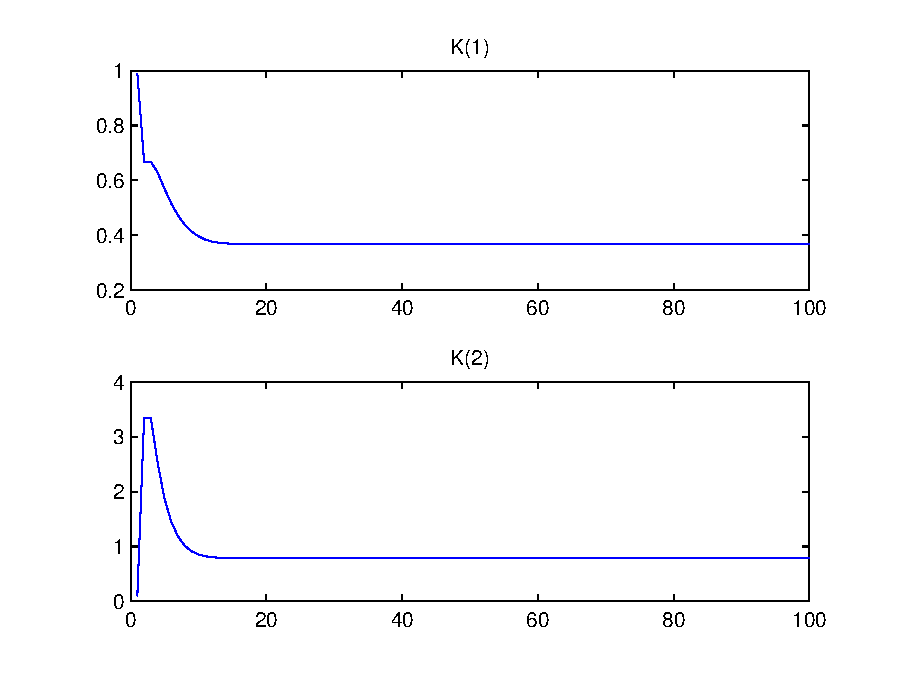
\includegraphics[width=.43\textwidth]{figures/norm_kalman}
          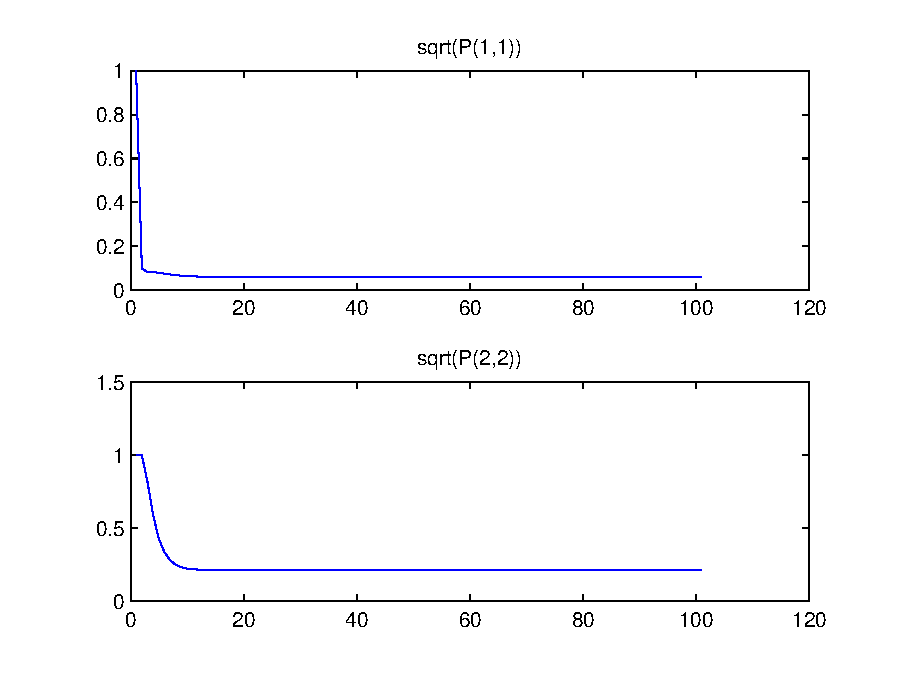
\includegraphics[width=.43\textwidth]{figures/norm_covar}
          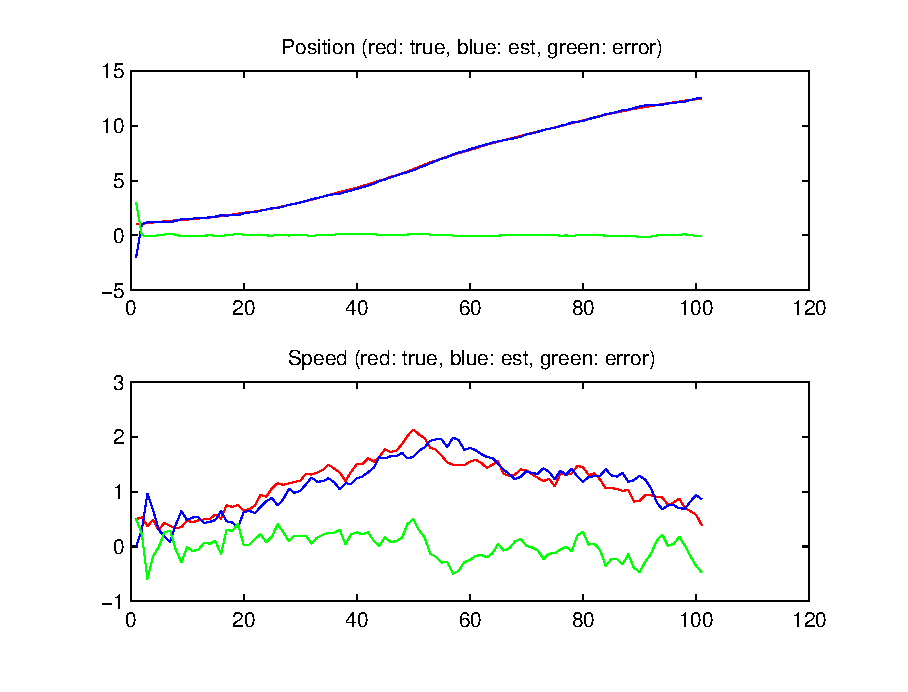
\includegraphics[width=.43\textwidth]{figures/norm_error}
        }
      }\\
      \subfloat[High process noise: $Q\times100, R$]{
        \centerline
        {
          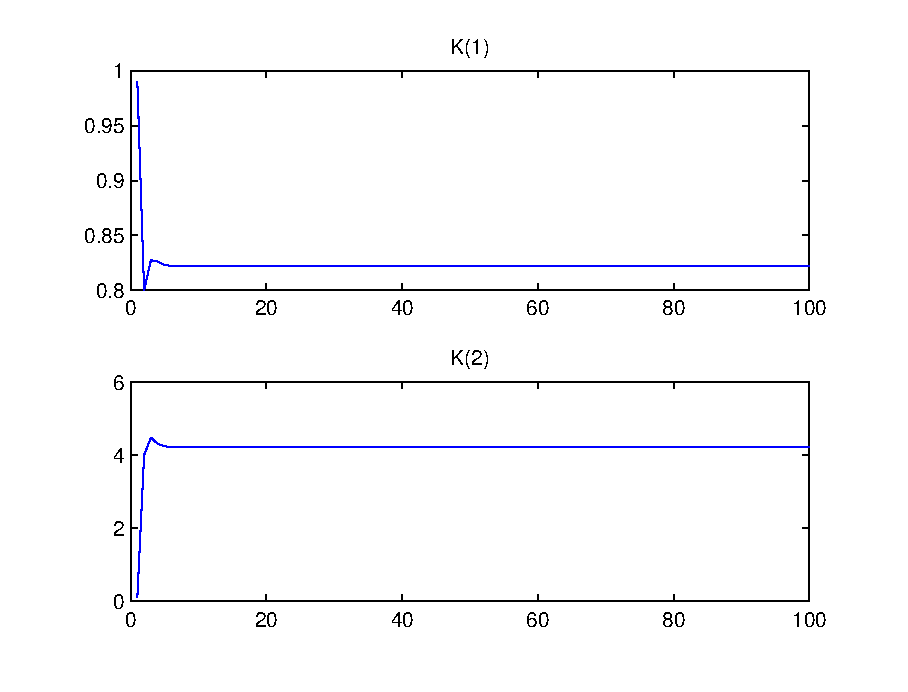
\includegraphics[width=.43\textwidth]{figures/highq_kalman}
          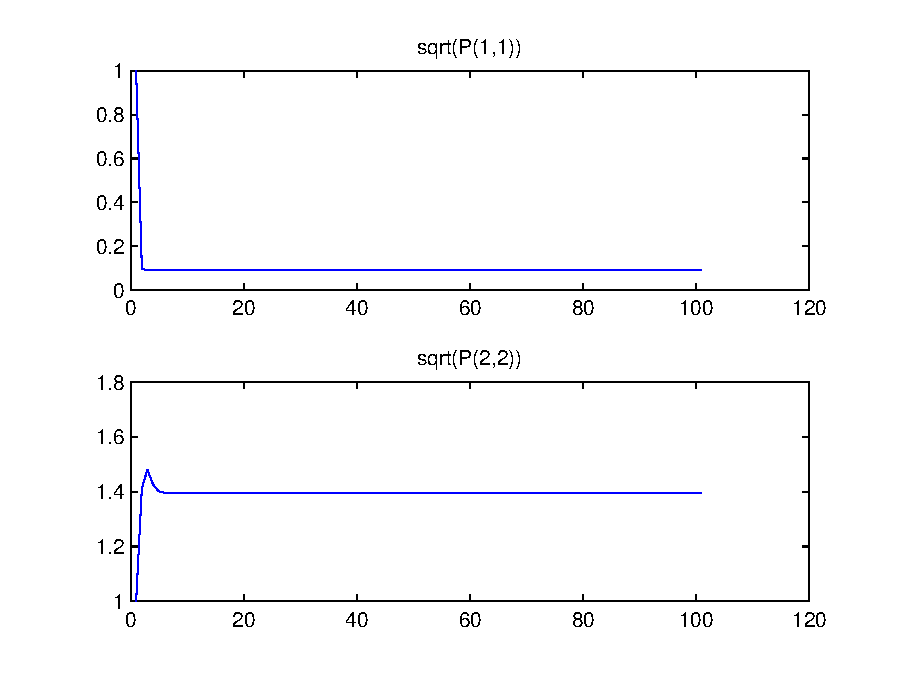
\includegraphics[width=.43\textwidth]{figures/highq_covar}
          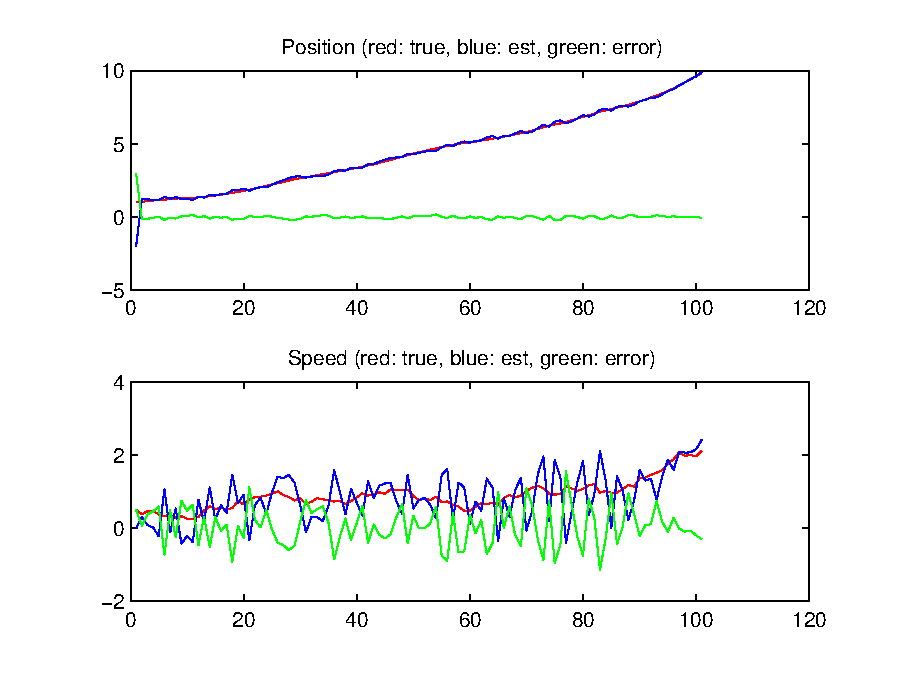
\includegraphics[width=.43\textwidth]{figures/highq_error}
        }

      }\\
      \subfloat[Low process noise: $Q/100, R$]{
        \centerline
        {
          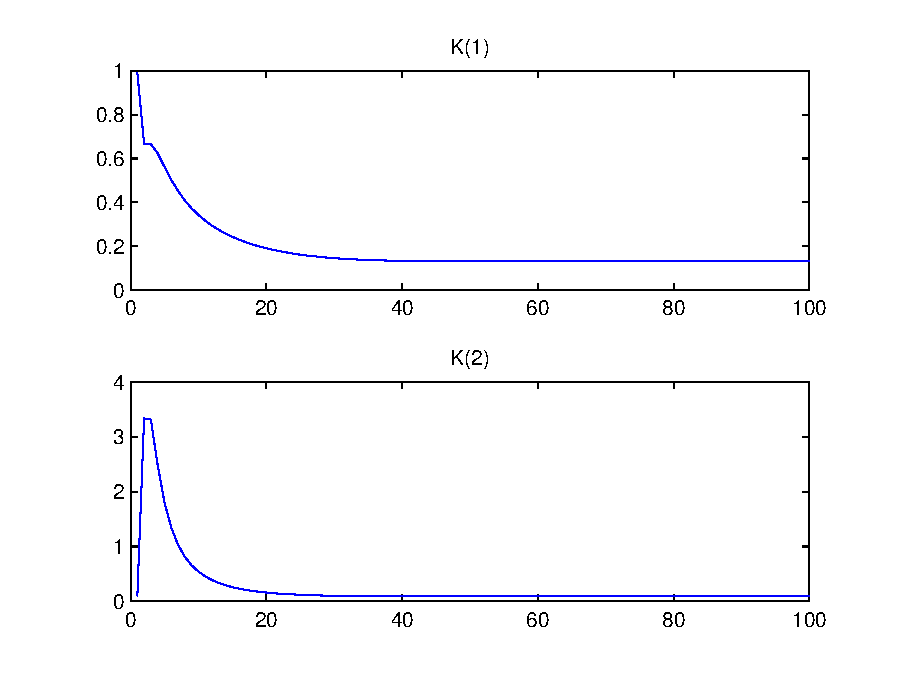
\includegraphics[width=.43\textwidth]{figures/lowq_kalman}
          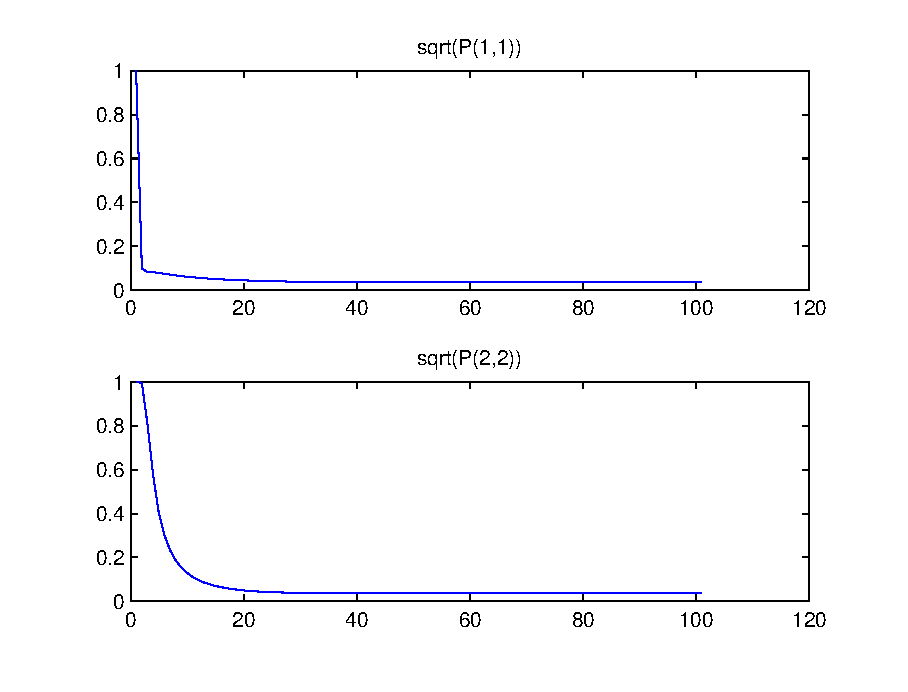
\includegraphics[width=.43\textwidth]{figures/lowq_covar}
          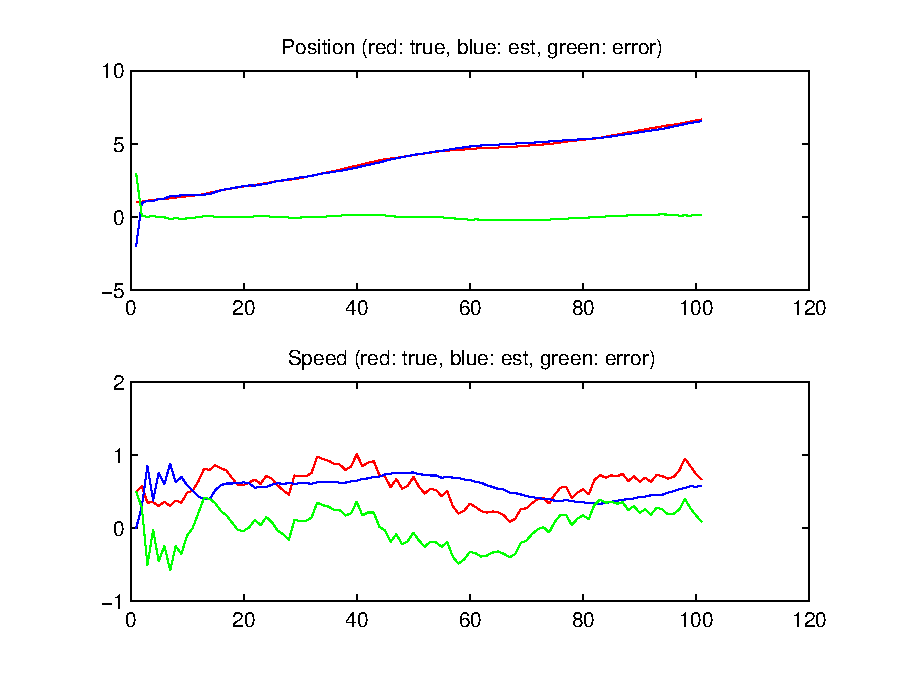
\includegraphics[width=.43\textwidth]{figures/lowq_error}
        }

      }\\
      \subfloat[High measurement noise: $Q, R\times100$]{
        \centerline
        {
          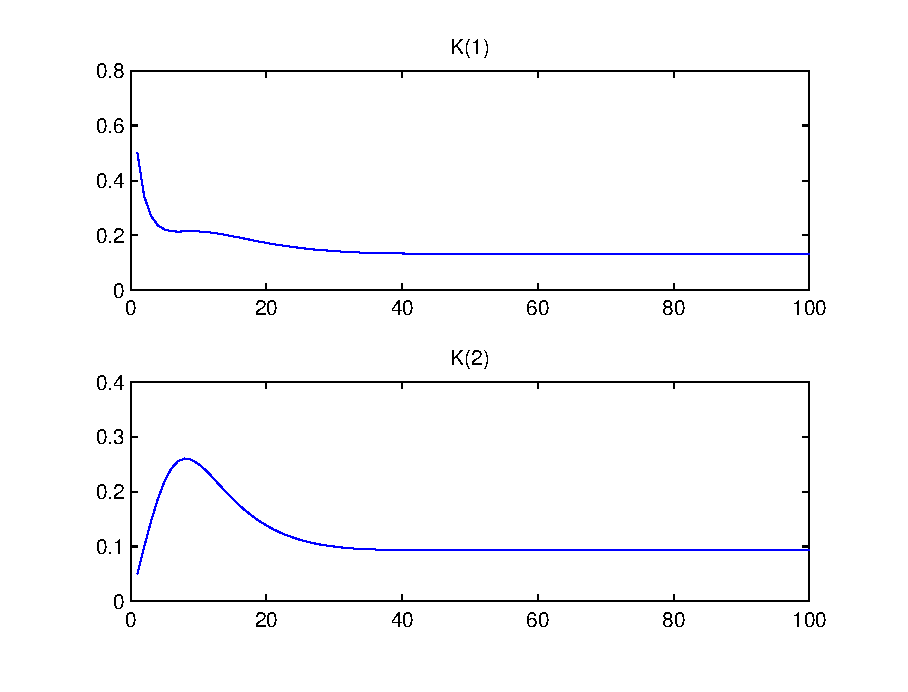
\includegraphics[width=.43\textwidth]{figures/highr_kalman}
          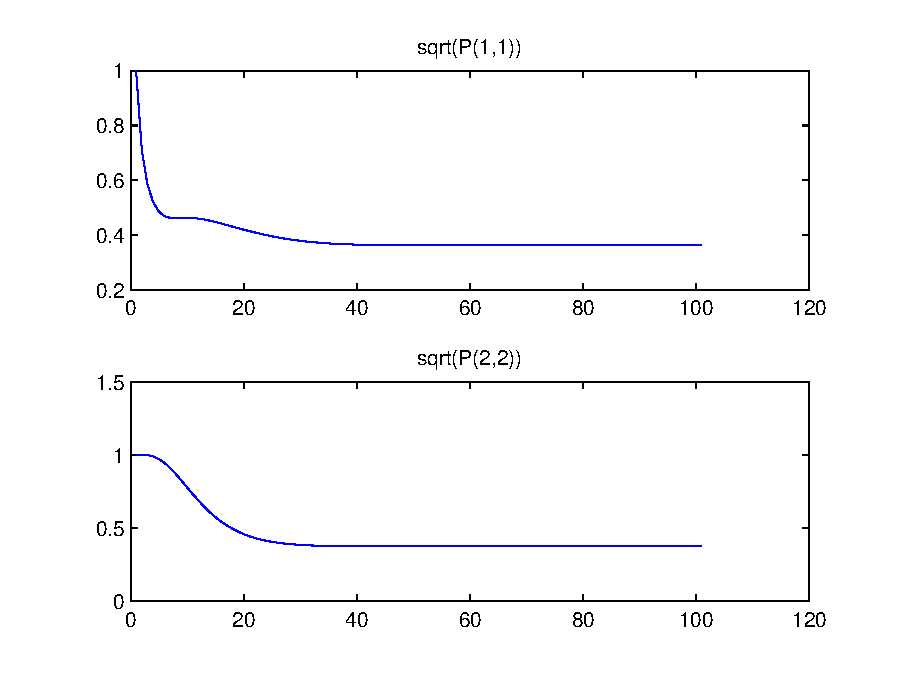
\includegraphics[width=.43\textwidth]{figures/highr_covar}
          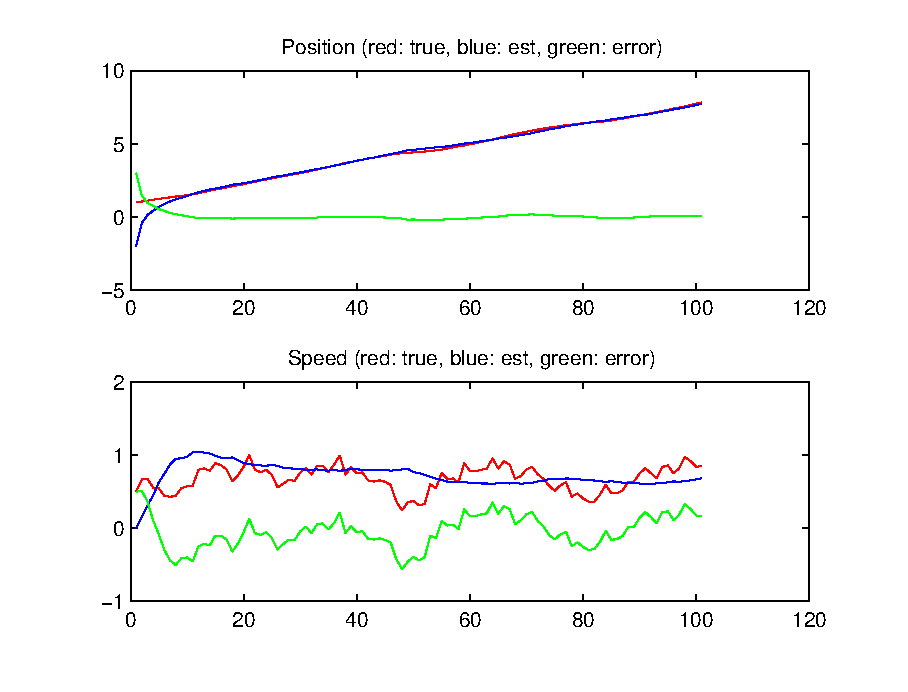
\includegraphics[width=.43\textwidth]{figures/highr_error}
        }

      }
      \caption{Graphs for different process and measurement noise models, from
        left to right the Kalman gain, covariance and error.}
  \end{figure}
  \begin{figure}
    \renewcommand{\figurename}{Figure (cont.)}
    \ContinuedFloat
      \subfloat[Low measurement noise: $Q,R/100$]{
        \centerline
        {
          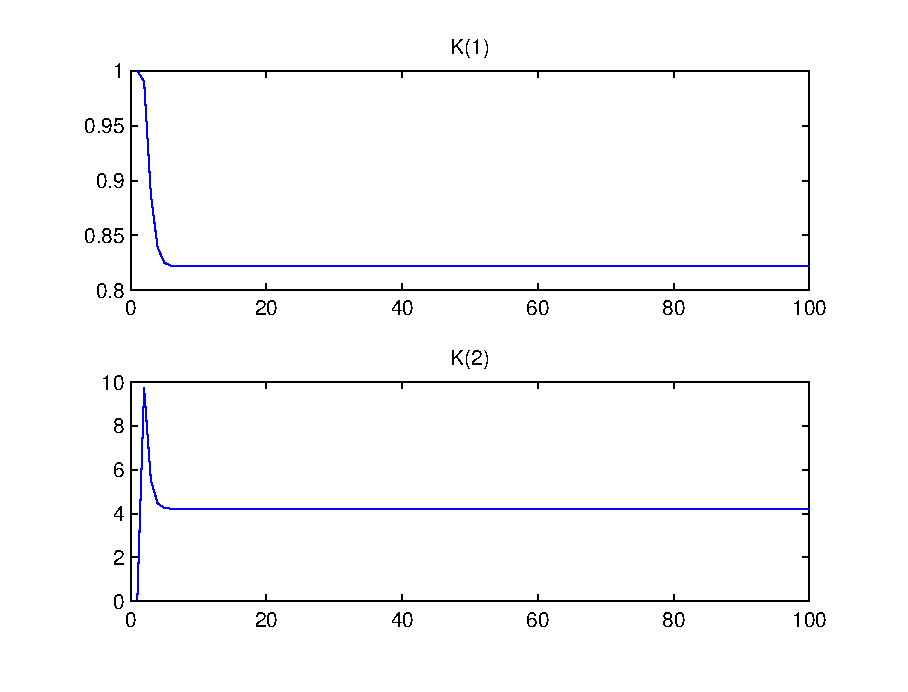
\includegraphics[width=.43\textwidth]{figures/lowr_kalman}
          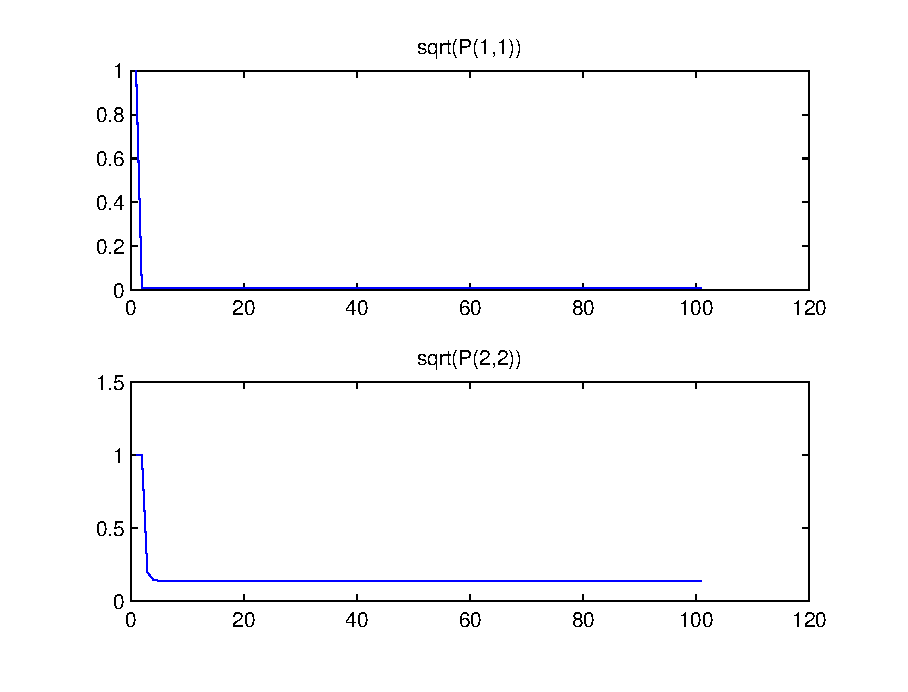
\includegraphics[width=.43\textwidth]{figures/lowr_covar}
          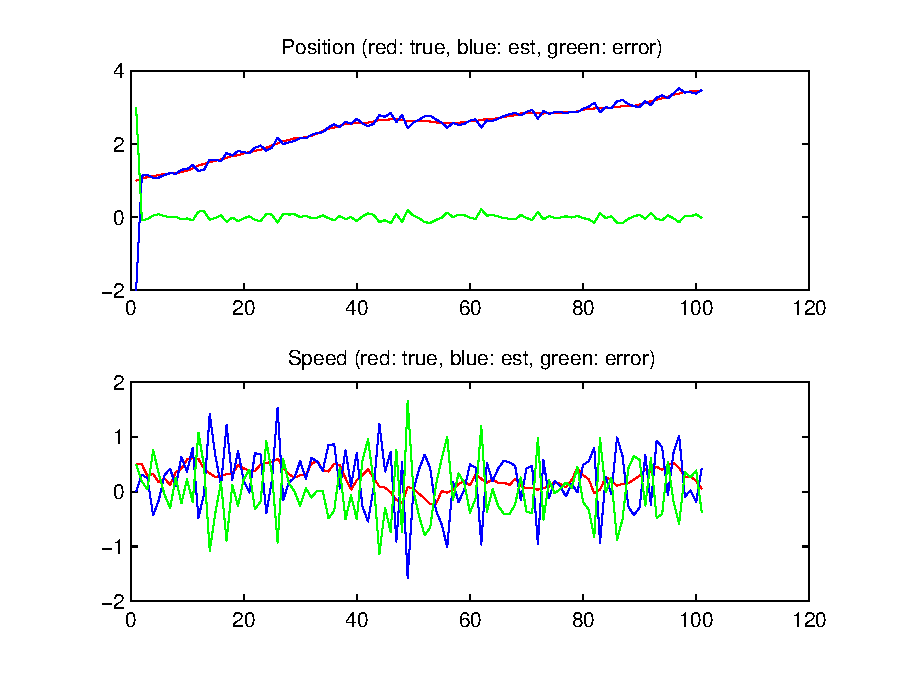
\includegraphics[width=.43\textwidth]{figures/lowr_error}
        }
      }
      \caption{Graphs for different process and measurement noise models, from
        left to right the Kalman gain, covariance and error.}
  \end{figure}
\item Changing the value of $P$ and $\hat{x}$ has no noticeable effect on the
  standard deviation of the error in position or velocity. However, making $P$
  very small, so that the uncertainty at the start is low, makes the time to
  convergence increase in the case of the position. Convergence for the velocity
  seems to take approximately the same amount of time. Making the uncertainty
  very large seems to have no effect on convergence or error.
\end{enumerate}
\newpage
\subsection{EKF Localisation}
\begin{enumerate}[resume]
\item The prediction step is used to generate the prior $\overline{bel}(x_t)$,
  which is our belief about the state of the robot before the measurements are
  taken into account. The update step integrates $\overline{bel}(x_t)$ and the
  probability of making the observed measurement.
  \begin{align}
    \overline{bel}(x_t)&=\int{p(x_t \mid
      u_{1:t},x_{t-1})bel(x_{t-1})dx_{t-1}}\\\eqname{Prediction step} \\
    bel(x_t)&=\eta p(z_t \mid x_t,M)\overline{bel}(x_t)\\\eqname{Update step}\\
    p(x_t\mid u_{1:t},z_{1:t},\bar{x}_0,M)&=\eta p(z_t \mid x_t,M)\underbrace{\int{p(x_t \mid
      u_t,x_{t-1})p(x_{t-1} \mid
      z_{1:t-1},u_{1:t-1},\bar{x}_0,M)dx_{t-1}}}_\text{Prediction Step}\label{eq:q5-3}
  \end{align}
  In \eqref{eq:q5-3}, the integral is equivalent to $\overline{bel}(x_t)$, and forms
  the prediction step. Multiplying this by the normalisation constant and
  measurement probability $\eta p(z_t \mid x_t,M)$ gives the update step.
\end{enumerate}
\section{Results}

\end{document}
